% !TEX TS-program = pdflatex
% !TEX encoding = UTF-8 Unicode

% This is a simple template for a LaTeX document using the "article" class.
% See "book", "report", "letter" for other types of document.

\documentclass[11pt]{article} % use larger type; default would be 10pt

\usepackage[utf8]{inputenc} % set input encoding (not needed with XeLaTeX)

%%% Examples of Article customizations
% These packages are optional, depending whether you want the features they provide.
% See the LaTeX Companion or other references for full information.

%%% PAGE DIMENSIONS
\usepackage{geometry} % to change the page dimensions
\geometry{letterpaper} % or letterpaper (US) or a5paper or....
\geometry{margin=1in} % for example, change the margins to 2 inches all round
% \geometry{landscape} % set up the page for landscape
%   read geometry.pdf for detailed page layout information

\usepackage{graphicx} % support the \includegraphics command and options

\usepackage[parfill]{parskip} % Activate to begin paragraphs with an empty line rather than an indent

%%% PACKAGES
%\usepackage{booktabs} % for much better looking tables
\usepackage{array} % for better arrays (eg matrices) in maths
%\usepackage{paralist} % very flexible & customisable lists (eg. enumerate/itemize, etc.)
\usepackage{verbatim} % adds environment for commenting out blocks of text & for better verbatim
%\usepackage{subfig} % make it possible to include more than one captioned figure/table in a single float
% These packages are all incorporated in the memoir class to one degree or another...
\usepackage{hyperref}

%%% HEADERS & FOOTERS
\usepackage{fancyhdr} % This should be set AFTER setting up the page geometry
\pagestyle{fancy} % options: empty , plain , fancy
\renewcommand{\headrulewidth}{0pt} % customise the layout...
\lhead{}\chead{}\rhead{}
\lfoot{}\cfoot{\thepage}\rfoot{}

%%% END Article customizations


%%% The "real" document content comes below...

\title{Pulse width modulation and timers}
\author{}
\date{} % Activate to display a given date or no date (if empty),
         % otherwise the current date is printed 

\begin{document}
\maketitle

%\begin{quote}
%Wise quote here.\\ \hbox{}\hfil -- {\em A Wise One}
%\end{quote}

\section{Introduction}

Up to now, all the communications with the Arduino have used digital interfaces. Reading the state of the light sensor. Activating a solenoid. Lighting an LED. Here, you will explore how the ATmega328 emulates \emph{analog outputs}, voltages that range between 0 -- 5 V.

The ATmega328 is not actually capable of producing a true analog signal. While there are microcontrollers that do have on-board digital-to-analog converters, the ATmega328 can only produce 0V or 5V signals -- not 3V, or 1.8V, or anywhere else in between. Instead, the chip uses a common technique called \emph{pulse width modulation}, or simply PWM, to \emph{mimic} analog voltages. In short, the microcontroller toggles a pin between 0V and 5V at a very high frequency so that the \emph{average} voltage approximates the desired voltage. By changing the \emph{duty cycle}, the proportion of the time that the pin is \verb|HIGH|, the apparent voltage can be controlled very precisely. For many devices -- motors, LEDs, and so forth -- the switching occurs so fast that it has no practical difference from a true analog voltage.

The machinery to produce PWM signals can be complicated -- it involves setting several control registers -- but Arduino has created a convenient function, \verb|analogWrite()|, to make PWM easy. Still, in this lab you’ll see how you can change frequencies, and use that knowledge to create different tones with a piezo buzzer, which will serve as the alarm for your alarm system.

\subsection{Objectives}

Upon successful completion of this lab, the student will be able to:
\begin{itemize}
\item Implement PWM using Arduino libraries and direct control,
\item Produce square waves of different frequencies, and
\end{itemize}

\section{Background materials}

Before coming to lab, the student should review the following materials:

\begin{itemize}
\item \emph{Pulse width modulation.} Everything you need to know should be included below.
\end{itemize}
{\bf Each student must complete the Pre-lab Worksheet and turn it in at the start of lab.}

\subsection{Timers}

There are six pins on the Arduino that are capable of create a PWM signal, indicated with a $\sim$ next to the pin. Each of three internal timers controls two of the pins, as shown in Table~\ref{tab:timers}, which also indicates the size of the timer (number of bits) for reference.

\begin{table}[h]
\centering
\begin{tabular}{c|c|c|c}
Timer & N (bits) & pin A & pin B \\
\hline\hline
0&8&6&5\\
\hline
1&16 &9&10\\
\hline
2&8&11&3\\
\hline
\end{tabular}
\caption{Timers on the ATmega328.}
\label{tab:timers}
\end{table}

\verb|Timer0| and \verb|Timer2| are \emph{8-bit} timers and \verb|Timer1| is a \emph{16-bit} timer. The size of the timer will affect the range of frequencies that you can create with it. As described in class, the timers each have an independent \emph{pre-scaler} that is used to set how fast the timer counts. If the pre-scaler is set to 1, the timer will increment by 1 for each tick of the system clock. Since the clock on the Arduino runs at 16 MHz, this means it will take an 8-bit timer $256 / 16 MHz = 16 \mu s$ to roll-over. By setting the pre-scaler to 8, it will take 8 ticks of the system clock to increment the timer by 1. As such it will take an 8-bit timer $256 \times 8 / 16 MHz = 256 \mu s$ to roll-over. For an N-bit timer, the general formula for calculating the rollover period, $\Delta T$ is

\[
\Delta T = \frac{2^N \times P}{f_{sys}}
\]
where $P$ is the pre-scaler and $f_{sys}$ is the frequency of the system clock. Alternatively, the rollover \emph{frequency} is given by $f_{timer} = 1/\Delta T$, or

\begin{equation}
f_{timer} = \frac{f_{sys}}{2^N \times P}
\label{eq:freq}
\end{equation}

When using the timer for PWM, the duty cycle is changed by setting a compare value, \verb|OCRnx|, where \verb|n| is the timer (0, 1, or 2) and \verb|x| is one of the two pins connected to that timer, A or B. In Fast PWM mode, the timer counts up from $0 \rightarrow 2^N-1$ and then rolls back over to $0$. Whenever it rolls over, it sets the corresponding pin to \verb|HIGH| and when it reaches 1 greater than the compare value, it switches the pin back to \verb|LOW|. Thus, for an N-bit timer, the duty cycle can be calculated as:

\begin{equation}
duty cycle= \frac{OCRnx + 1}{2^N}
\label{eq:duty.cycle}
\end{equation}

When you call \verb|analogWrite(<pin>, <value>)|, all the Arduino library does is set the compare value, \verb|OCRnx|, to \verb|<value>|. Note that passing 0 to \verb|analogWrite(<pin>, <value>)| would normally produce a small, but non-zero duty cycle; however, the Arduino library has an exception for that case where it sets the pin to \verb|LOW| and turns off the PWM function so that the functionality is more intuitive.

\subsection{Changing frequencies}

Changing the pre-scaler alone would not give much control over the timer frequency. To make sounds of different frequencies, it is useful to have finer control over the frequency. Indeed, fine-scale control can be achieved by running the timer in CTC mode, which is short for Clear Timer on Compare Match. In CTC mode, the timer rolls over at a specific value, the \verb|TOP| value. The general formula then becomes:

\[
f_{timer} = \frac{f_{sys}}{(TOP + 1) \times P}
\label{eq:top}
\]

where the $+1$ is there because it takes an extra timer increment to get from \verb|TOP| back to 0. In CTC mode, you can set a pin to toggle every time the timer rolls over, which will produce a square wave. Connecting the pin to a speaker (or piezo buzzer) will cause it to make a sound. Note that if you toggle a pin on rollover, the frequency will be half that of the timer, because it will either be \verb|HIGH| or \verb|LOW| for each timer cycle. When in CTC mode, \verb|TOP| is set using \verb|ORCnx|, which shouldn’t be confused with it’s functionality in the previous section.

\section{In lab}

\subsection{Pulse width modulation}
\label{sec.analout}

\subsubsection*{Procedure}
\begin{enumerate}
\item Construct the circuit shown in Figure~\ref{fig:led.pwm}. Use Equation~\ref{eq:duty.cycle} to calculate the theoretical duty cycle and record it in Table~\ref{tab:duty.cycle} for each of the values there.

\begin{figure}[htbp]
\begin{center}
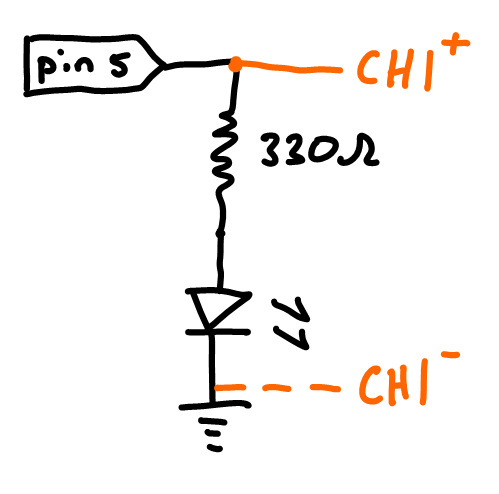
\includegraphics[width=2.5in]{figures/led5}
\caption{Yet another LED circuit. Be sure to use pin 5.}
\label{fig:led.pwm}
\end{center}
\end{figure}

\item Write a program that declares pin 5 as an \verb|OUTPUT| and sends a PWM command to it using \verb|analogWrite()|. In the \verb|loop()|, print the value in \verb|OCR0B| once per second -- you may use \verb|delay()|.
\item For each value in Table~\ref{tab:duty.cycle}, change the value that is passed to \verb|analogWrite()| and run the code. Connect your oscilloscope to the output of pin 5 and set the trigger to capture the rising edge. Adjust the time scale until you can see four or five PWM cycles. Dig through the built-in measurements until you find ``Duty cycle'' and compare the measured duty cycle to the theoretical value. Complete the table.
\begin{table}[h]
\centering
\begin{tabular}{c|c|c|c|c}
PWM Value & Exp. Duty Cycle & Act. Duty Cycle & Avg. Voltage & Perceived Brightness\\
\hline\hline
0&&&&\\
\hline
50&&&&\\
\hline
100&&&&\\
\hline
150&&&&\\
\hline
200&&&&\\
\hline
255&&&&\\
\hline
300&&&&\\
\hline
\end{tabular}
\caption{Table for PWM values.}
\label{tab:duty.cycle}
\end{table}

\item What happens to the LED when you pass 300 as the PWM parameter? Does it glow brightly? What is the measured duty cycle? Explain.
\vspace{1in}

\item Instead of using \verb|analogWrite()|, change your code to read:
\begin{verbatim}
     OCR0B = 75;
\end{verbatim}
What is the duty cycle? Is this what you expect?

\vspace{0.5in}
\item Use your oscilloscope to determine the frequency of the PWM signal. Knowing that pin 5 is controlled by \verb|Timer0|, an 8-bit timer, determine what pre-scaler is being used by the Arduino library using Equation~\ref{eq:freq}.

\vspace{0.5in}
\item Add a line to your \verb|setup()| function to print the \verb|TCCR0B| register to the Serial Monitor,

\begin{verbatim}
     Serial.println(TCCR0B, HEX);
\end{verbatim}

The last three bits of this register control the pre-scaler for \verb|Timer0|. Consult the pages posted on collab (TCCR0B.pdf) to check what the bits correspond to. Do they agree?
%\item In your \verb|setup()| routine, add code to change the prescaler to 256; Make sure you don’t clobber any of the other bits in \verb|TCCR0B|! You can either change the bits using bit manipulators or, using the value you printed in the previous step, figure out what the complete value of \verb|TCCR0B| should be and set it directly. What frequency do you expect the signal to be? What is it?
%\item Do you notice anything about the rate at which the \verb|loop()| executes? Can you think of why this might be?
\end{enumerate}

{\bf Demonstrate your working system to an instructor!}

\subsection{Sounds}

Arduino does have a \verb|Tone| library, but not only is it more cumbersome than it needs to be\footnote{Stupidly cumbersome, if you ask me.}, it is useful for you to understand how to fine-tune the frequency of a timer manually. In this section, you’ll use the 16-bit \verb|Timer1|, which gives you a huge range of frequencies, including the painful ones above 10 kHz. You’ll use a piezo buzzer to make the sounds.

\subsubsection*{Procedure}
\begin{enumerate}
\item Build the circuit shown in Figure~\ref{fig:piezo}. The \href{http://cdn.sparkfun.com/datasheets/Components/General/cem-1203-42-.pdf}{\underline{datasheet}} indicates that the piezo is meant to be driven using 3.3V -- since the Arduino outputs 5V from each pin, you’ll use a low-side driver. Size the resistor, R, using the rules-of-thumb for a low-side driver. Connect the oscilloscope as shown.

\begin{figure}[htbp]
\begin{center}
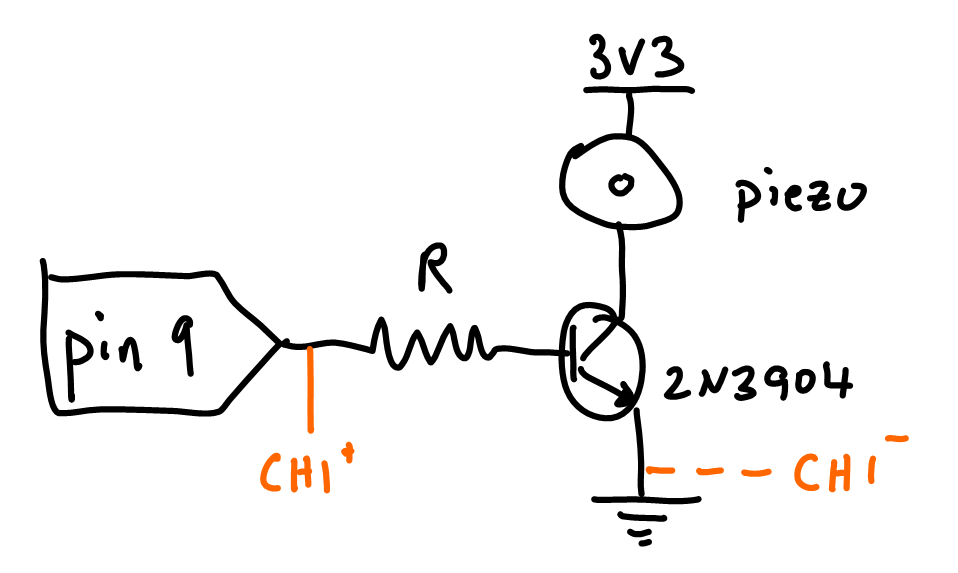
\includegraphics[width=4in]{figures/piezo}
\caption{Circuit for the piezo element.}
\label{fig:piezo}
\end{center}
\end{figure}

\item Wire a standard button to whichever pin you’d like and edit the code appropriately.
\item Download \verb|jammin_tunes.ino| from collab. The \verb|setup()| function sets up \verb|Timer1| to run in CTC mode. There are comments in the code. Use the \verb|Button| class you made last week to activate and deactivate the piezo. Use Equation~\ref{eq:freq} to determine the frequency.
\item Run the program. Press the button to turn on and off the piezo. Use the oscilloscope to determine the frequency. Do they agree?
\item Using Equation~\ref{eq:top}, calculate the value of \verb|TOP| needed to create a tone with a frequency of 440 Hz (middle A) and set \verb|OCR1A| to one less than the value you calculated.
\item Run the new program an verify that the frequency is correct.
\end{enumerate}

{\bf Demonstrate your working system to an instructor!}

\clearpage

\subsection{Pre-lab worksheet}
\label{sec:prelab}

{\bf To be turned in at the start of lab.} Completed individually, but you are welcome to talk to others about the material.

\emph{Answers with incomplete or incorrect units will be marked as wrong!}

\begin{enumerate}
\item Give three reasonably distinct examples of where an analog output might be useful.
\vspace{1in}
\item What is the duty cycle of a PWM signal created with the statement \verb|analogWrite(5, 42);|?
\vspace{1in}
\item What is the frequency of an 8-bit timer on an Arduino Uno if the prescaler is 8 and \verb|TOP| is set to 199?
\vspace{1in}
\end{enumerate}
\end{document}

